\documentclass[tikz,border=7pt]{standalone}
\usepackage{amsmath}
\usetikzlibrary{arrows.meta}

\definecolor{ink}{HTML}{21352F}
\definecolor{teal}{HTML}{087F7B}
\definecolor{rose}{HTML}{B65A62}
\definecolor{gold}{HTML}{C58B2A}
\definecolor{blue}{HTML}{4B77A8}

\begin{document}
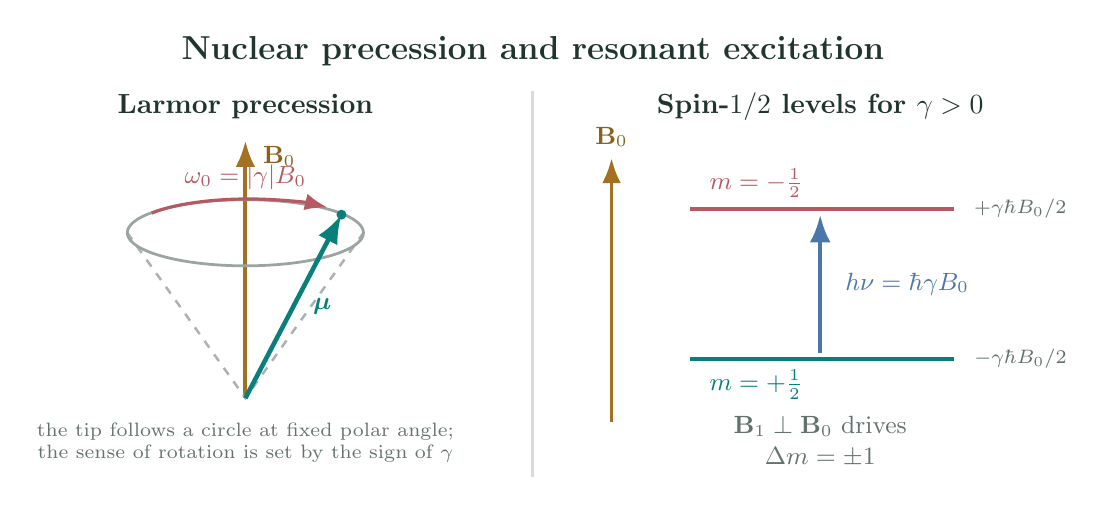
\begin{tikzpicture}[font=\sffamily,>=Latex]
  \node[font=\bfseries\large,text=ink] at (0,2.95)
    {Nuclear precession and resonant excitation};

  % Classical motion: fixed polar angle, circular path of vector tip.
  \node[font=\bfseries,text=ink] at (-3.65,2.25)
    {Larmor precession};
  \coordinate (O) at (-3.65,-1.45);
  \draw[->,line width=1.45pt,draw=gold!82!black]
    (O) -- (-3.65,1.82);
  \node[anchor=west,text=gold!70!black,font=\small]
    at (-3.55,1.62) {$\mathbf B_0$};

  \draw[dashed,draw=ink!38,line width=0.9pt]
    (-5.15,0.65) -- (O) -- (-2.15,0.65);
  \draw[draw=ink!45,line width=1pt]
    (-3.65,0.65) ellipse [x radius=1.5,y radius=0.42];
  \draw[->,line width=1.65pt,draw=teal]
    (O) -- (-2.43,0.88)
    node[midway,right=3pt,text=teal,font=\small]
    {$\boldsymbol{\mu}$};
  \fill[teal] (-2.43,0.88) circle (1.8pt);

  \draw[->,line width=1.15pt,draw=rose]
    (-4.84,0.90)
    arc[start angle=145,end angle=48,x radius=1.5,y radius=0.42];
  \node[text=rose,font=\small] at (-3.65,1.35)
    {$\omega_0=\lvert\gamma\rvert B_0$};
  \node[align=center,text=ink!70,font=\scriptsize] at (-3.65,-2.02)
    {the tip follows a circle at fixed polar angle;\\
     the sense of rotation is set by the sign of $\gamma$};

  \draw[ink!18,line width=1pt] (0,-2.45) -- (0,2.45);

  % Quantum spin-1/2 levels for gamma > 0.
  \node[font=\bfseries,text=ink] at (3.65,2.25)
    {Spin-$1/2$ levels for $\gamma>0$};
  \draw[->,line width=1.35pt,draw=gold!82!black]
    (1.0,-1.75) -- (1.0,1.6)
    node[above,text=gold!70!black,font=\small] {$\mathbf B_0$};

  \draw[line width=1.55pt,draw=rose] (2.0,0.95) -- (5.35,0.95);
  \node[anchor=west,text=rose,font=\small] at (2.12,1.28)
    {$m=-\tfrac12$};
  \node[anchor=west,text=ink!72,font=\scriptsize] at (5.48,0.95)
    {$+\gamma\hbar B_0/2$};

  \draw[line width=1.55pt,draw=teal] (2.0,-0.95) -- (5.35,-0.95);
  \node[anchor=west,text=teal,font=\small] at (2.12,-1.28)
    {$m=+\tfrac12$};
  \node[anchor=west,text=ink!72,font=\scriptsize] at (5.48,-0.95)
    {$-\gamma\hbar B_0/2$};

  \draw[->,line width=1.55pt,draw=blue]
    (3.65,-0.88) -- (3.65,0.88)
    node[midway,right=5pt,text=blue,font=\small]
    {$h\nu=\hbar\gamma B_0$};
  \node[align=center,text=ink!70,font=\small] at (3.65,-2.0)
    {$\mathbf B_1\perp\mathbf B_0$ drives\\$\Delta m=\pm1$};
\end{tikzpicture}
\end{document}
